\chapter{Introduction\label{ch:intro}}
 
Soot is a carbonaceous product formed from the incomplete combustion of hydrocarbon fuels. Although soot may appear as a dark cloud or plume to the naked eye, it is actually a collection of nanoscale particles, as shown in \cref{fig:intro:dieselsoot}. Soot particles are required to increase the radiant energy of flames in furnaces and boilers, but they are also an undesired waste product in many engineering systems such as internal combustion engines, gas turbine combustors, and combustion-based power plants. If released into the atmosphere, soot can contribute to haze, global warming, and acid rain. Exposure to these particles results in an increased risk for a variety of ailments including strokes~\cite{popeiii2006}, atherosclerosis~\cite{polichetti2009,kennedy2007,popeiii2006}, lung cancer~\cite{kennedy2007,popeiii2006}, and cardiovascular mortality~\cite{polichetti2009,kennedy2007,popeiii2006}, and these adverse health effects have been observed to be closely related the number, composition, and size of particles rather than their mass~\cite{seaton1995,lighty2000}. While the fate of federal regulations for particulate matter under the current administration of President Donald J. Trump is unclear, these regulations are expected to become more stringent in the coming decades. 

\begin{figure}[htb]
  \centering
  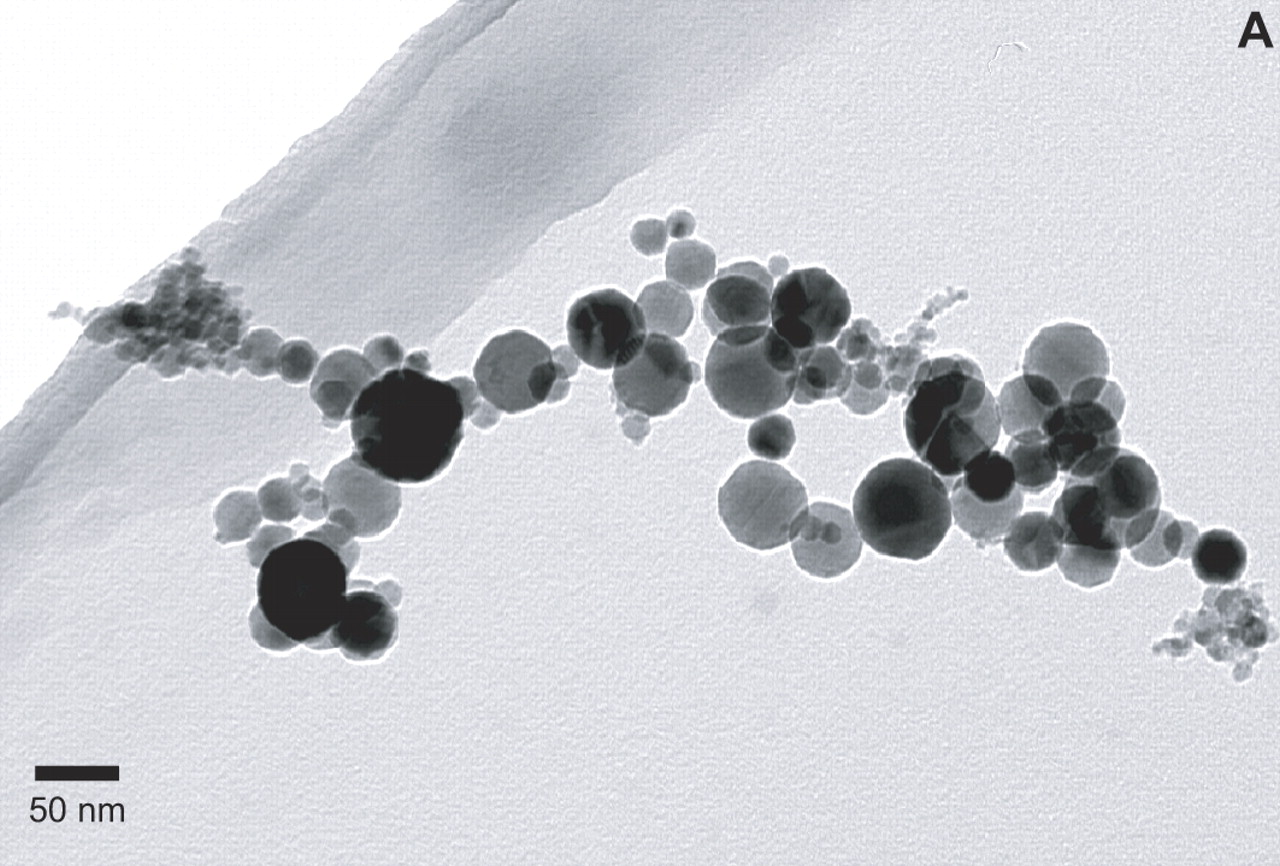
\includegraphics[width=0.4\linewidth]{ch-intro/figures/diesel-soot}
  \caption[Soot From Diesel Car Engine]{Transmission Electron Microscope (TEM) image of soot collected from the exhaust of a diesel car engine. Reproduced from Grob\'ety \etal~\cite{grobety2010}.}
  \label{fig:intro:dieselsoot}
\end{figure}

The production of next-generation, environmentally friendly combustion systems will depend on numerical simulation for rapid design optimization. The task of predicting how soot evolves in the turbulent reacting flows of these systems is nontrivial and will require high-fidelity models for soot, combustion, and turbulence. The large range of spatial and temporal scales present in these systems makes the development of each component model extremely challenging. Furthermore, integration into a single framework necessitates accounting for the interactions between models. The preferred framework to design these low emissions systems is Large Eddy Simulation (LES), a computationally efficient approach where the large, geometry-dependent scales of the system are resolved and the small scales are modeled. Today's state-of-the-art simulations have progressed towards achieving this goal, but significant work still lies ahead.

The overall objective of this thesis is to advance the understanding of how turbulence affects the dynamics of soot. Specifically, the small-scale interactions between soot, chemistry, and turbulence as well as the transport of species in turbulent nonpremixed combustion are analyzed. The insights that are gained are used to develop models for LES. A survey of previous investigations on both topics is presented in the upcoming sections, but first, a brief overview of the processes that guide the evolution of soot is provided.


%% ***
%% My rough idea for intro:
%% What is soot and why it needs to be studied/modeled
%% Explanation of dynamics of soot/various modes of evolution

%% Goal is to motivate need for ZASSP (closure model for soot transport equation SOOT MODEL that accounts for spatial intermittency of soot (soot-turbulence interactions) as well as its interaction/connection to combustion chemistry). Also need to motivate need for SSTA (transport approach that uses the nonpremixed flamelet framework TURBULENT COMBUSTION MODEL WITH EMPHASIS ON SOOT PRECURSORS with differential diffusion, transporting species with relatively slow chemistry with molecular diffusion and species with fast chemistry with unity effective Lewis numbers).

%% SOOT-TURBULENCE-CHEMISTRY INTERACTIONS:
%% Effects of turbulence on soot, experimental evidence of influence of strain
%% Previous modeling attempts of soot evolution in turbulent combustion: RANS, LES, DNS (highlight findings and weaknesses)
%% Explain how the model I developed will address these deficiencies

%% EFFECT OF TRANSPORT ON SOOT EVOLUTION:
%% Mention species that influence soot evolution and dictate flame structure have a variety of molecular weights and scales.
%% Somehow incorporate experimental findings into this section
%% Previous modeling attempts for transport of species in turbulent combustion (highlight findings and weaknesses, especially with consideration of soot)
%% Explain how the turbulent combustion transport model will address these deficiencies
%% ***

\section{Dynamics of Soot}
\label{sec:intro:dynamics}
%\section{Modeling Framework for Large Eddy Simulation}
%\label{sec:intro:framework}

%% Summarize previous works on soot and turbulent combustion models as well as other closure approaches other than the presumed PDF approach.

%% There are three classes of statistical models that are generally utilized. The most accurate is the Monte Carlo (MC) approach, where a large population of notional particles is used to represent the NDF. The evolution of these particles is determined by assuming that all aerosol processes are governed by stochastic processes~\cite{balthasar2003} or that only the coagulation of particles occurs stochastically~\cite{lucchesi2017}. MC is able to capture the NDF with high accuracy, as thousands of internal coordinates can be used to provide highly detailed descriptions of aggregate structure and chemical composition~\cite{celnik2008,mosbach2009}. However, the computational cost associated with such accuracy constrains the application of MC to simple configurations such as homogeneous reactors~\cite{celnik2007} and one-dimensional laminar premixed flames~\cite{patterson2007}. Additionally, explicitly coupling MC to the gas-phase chemistry is not straightforward~\cite{celnik2007}.

%% The second class of statistical models comprises sectional methods, where the NDF is discretized into bins and equations are solved for the number of particles in each bin. Like MC simulations, sectional methods provide accurate depictions of the complete NDF. However, as the number of internal coordinates used to describe the NDF increases, the associated computational cost can become intractable due to the required number of bins~\cite{gelbard1980}. Sectional methods do possess an advantage over MC, as they are deterministic and can be explicitly coupled to gas-phase chemistry.

The life of a soot particle begins with the formation of Polycyclic Aromatic Hydrocarbons (PAH). The exact mechanism for this process is not yet fully understood, but in general, large aliphatic fuel molecules are oxidized into smaller hydrocarbons by $\beta$-scission and \ce{H}-abstraction~\cite{law2006}. Further reactions eventually lead to the creation of species such as acetylene (\ce{C2H2}), propargyl (\ce{C3H3}), cyclopentadienyl (\ce{C5H5}), phenyl (\ce{C6H5}), and benzene (\ce{C6H6})~\cite{wang1997,richter2000,wang2011}. Benzene, the first aromatic ring, plays an important role in the production of multi-ring aromatic species. Larger PAH with molecular weights of 500-1000 amu are considered to be the immediate precursors of soot, and their formation can occur through the attachment of \ce{C2}, \ce{C3}, and other small units to benzene~\cite{wang1997,richter2000}. Growth is further fostered through the addition of PAH radicals and through reactions between PAH species, including PAH-PAH radical recombination and addition reactions~\cite{richter2000,wang2011}. Collisions between these gas-phase PAH lead to dimerization, and the collisions between PAH dimers form solid-phase nascent soot particles known as primary particles~\cite{frenklach1991,richter2000,schuetz2002,blanquart2009,wang2011}. This process can take several milliseconds~\cite{richter2000,wang2011} and is summarized in the first two frames of \cref{fig:intro:dynamics:sootdynamics}.

\begin{figure}[htb]
  \centering
  \includegraphics[width=\linewidth]{ch-intro/figures/soot-dynamics}
  \caption[Dynamics of Soot]{Various processes that govern the dynamics of soot.}
  \label{fig:intro:dynamics:sootdynamics}
\end{figure}

Once the first primary particles appear, their evolution is dictated by various physical and chemical processes. In the top right frame of \cref{fig:intro:dynamics:sootdynamics}, coagulation is depicted. During coagulation, the number density of particles decreases as existing particles collide and no mass is transferred from gas-phase species to solid-phase particles~\cite{kazakov1995,hmom2009}. There are two limits as to how coagulation can occur. In the limit of pure coalescence, a primary particle is assumed to undergo maximum deformation as it collides with another particle to form a larger spherical particle. This is facilitated by the liquid-like nature of nascent particles as noted in experimental studies~\cite{dobbins1998,dobbins2002}. In the limit of pure aggregation, the colliding particles do not deform and the total surface area is assumed to be preserved in the resulting particle.

Soot can also evolve through two different growth pathways, as shown in the bottom left and middle frames of \cref{fig:intro:dynamics:sootdynamics}. During condensation, a gas-phase PAH dimer collides with a soot particle and attaches to its surface~\cite{hmom2009,blanquart2009}. Surface growth, on the other hand, involves reactions with gas-phase acetylene. Carbon atoms are added to the surface of the soot particle through the \ce{H}-Abstraction \ce{C2H2}-Addition (HACA) mechanism~\cite{frenklach1985,frenklach1991}. Both growth processes influence soot morphology by rendering particles and aggregates more spherical~\cite{mitchell1998,mitchell2003,park2003}.

These growth modes are balanced by destructive modes, as illustrated in the bottom right frame of \cref{fig:intro:dynamics:sootdynamics}. Oxidation occurs when hydroxyl radicals (and molecular oxygen to a lesser extent) strip carbon atoms from the surfaces of soot particles, forming products such as \ce{CO} and \ce{CO2}~\cite{kazakov1995,neoh1981,stanmore2001}. Oxidation by hydroxyl radicals proceeds rapidly, but oxidation by molecular oxygen occurs slowly enough such that the internal structures of large aggregates are weakened. This leaves these aggregates susceptible to breaking apart in a process known as fragmentation~\cite{mueller2011,neoh1985}.

Clearly, the lifetime of soot is governed by interactions with species of various weights, length scales, and time scales. Accurately predicting the evolution of soot in a turbulent reacting flow requires accounting for these interactions as well as for the influence of the surrounding flow field. Previous research addressing these topics is surveyed in the upcoming sections.

\section{Soot-Chemistry-Turbulence Interactions}
\label{sec:intro:scti}

Discussion of previous works on subfilter modeling with respect to soot. Can discuss Monte Carlo approach, various method of moment approaches, etc.

\section{Effect of Transport on Soot Evolution}
\label{sec:intro:transport}

Can discuss various approaches to modeling transport for sooting flames. Can discuss diffusion between soot and gas-phase species (DNS paper by Jackie Chen).

Main points:
Discussion about soot PAH precursors and other strain-sensitive species.
Classical theory is that turbulence mixes indiscriminately at sufficiently high Re.
PAH are very sensitive to the local scalar dissipation rate due to their slow formation chemistry
DNS studies suggest PAH are confined to spatially intermittent regions of low scalar dissipation rate that are on the order of the Kolmogorov scale or smaller
At such scales, transport is governed by molecular diffusion
Pitsch and Peters flamelet equations with full differential diffusion
Wang's bimodal transport

\section{Organization of Thesis}
\label{sec:intro:org}

This thesis is organized as follows. In \cref{ch:lesmodels}, the foundation for modeling soot in LES of turbulent nonpremixed combustion is presented. In \cref{ch:subfilter}, the model for small-scale interactions between soot, combustion chemistry, and turbulence is developed and validated \textit{a priori} against a recent DNS database. In \cref{ch:transport}, the transport model for species with relatively slow formation chemistry is presented and validated \textit{a priori} with solutions to the flamelet equations. In \cref{ch:lesresults}, these models are implemented in LES and validated against experimental measurements from a series of three laboratory-scale flames. Finally, in \cref{ch:conclusion}, the results from this thesis are summarized and suggestions for future work are proposed.

The accomplishments and new contributions of this thesis are summarized below.
\begin{itemize}
\item \textbf{$Z$-Activated Soot Subfilter PDF (ZASSP):} Developed a presumed subfilter PDF model to close the filtered transport equations for the soot model. It contains a dependence on the mixture fraction to address the lack of soot in fuel-lean regions and has the form of a double-delta distribution to account for the high spatial intermittency of soot (Chapter 3).
\item \textbf{Strain-Sensitive Transport Approach (SSTA):} Developed a model that transports species governed by relatively slow formation chemistry with molecular diffusion and transports species governed by fast kinetics with equal effective diffusivities. A strain-sensitivity parameter is used to categorize each species (Chapter 4).
\item \textbf{Validation of the Integrated Large Eddy Simulation Model:} Conducted Large Eddy Simulations with ZASSP and SSTA for a series of three laboratory-scale ethylene-hydrogen-nitrogen simple jet flames (Chapter 5).
\end{itemize}



%% This documentclass, \texttt{puthesis.cls}, is setup for a Ph.D. dissertation for Princeton University. The Mudd Library website~\cite{mudd2009} provides detailed specifications for how to format your disseration~\cite{muddthesis2009}. Please review those documents, as the requirements may have changed since this template was created. Also, review the ProQuest Dissertation Guide~\cite{proquest2006}, which has additional formatting rules that are important for the submission of the electronic copy of your dissertation.

%% This template includes many details about the requirements and common practices for writing, printing, and submitting your dissertation. However, this is \textbf{NOT} an official document. It was written by Jeffrey Dwoskin and is current as of May 2010 based on requirements for the Electrical Engineering department, but the requirements may have changed. Please verify all information, deadlines, costs, requirements, and formatting rules with the Mudd Library website~\cite{mudd2009}, with the Graduate School, and with your department.

%This document serves as a template to demonstrate how to use the \texttt{puthesis} documentclass for a Princeton University Ph.D.\ Disseration. Some of the requirements for a master's thesis or an undergraduate thesis are different, especially the text on the title page, so you will need to make some modifications to use this template for those purposes. 

This template is setup to easily make a few different versions of your dissertation. The version you will print and have bound should generally be single spaced (and single-sided), and not contain any hyperlinks. The electronic version that you submit to your readers to review and to be published by ProQuest will be double spaced, and will contain PDF features such as bookmarks for each section and internal links to citations, footnotes, and other internal references.  

During the writing process, you may want to disable some of the frontmatter (list of tables, list of figures, acknowledgements, and maybe even the table of contents. I have not tested this template with equations or a list of symbols, but those are available.

